\documentclass{beamer}
\usetheme{Warsaw}
\usefonttheme{professionalfonts}
%\usefonttheme{serif}
%\usetheme{CambridgeUS}
%\usecolortheme{beaver}

% Add frame number and total frame number in footline
\defbeamertemplate*{footline}{shadow theme}{%
    \leavevmode%
    \hbox{\begin{beamercolorbox}[wd=.5\paperwidth,ht=2.5ex,dp=1.125ex,leftskip=.3cm plus1fil,rightskip=.3cm]{author in head/foot}%
            \usebeamerfont{author in head/foot}\hfill\insertshortauthor
        \end{beamercolorbox}%
        \begin{beamercolorbox}[wd=.4\paperwidth,ht=2.5ex,dp=1.125ex,leftskip=.3cm,rightskip=.3cm plus1fil]{title in head/foot}%
            \usebeamerfont{title in head/foot}\insertshorttitle\hfill%
        \end{beamercolorbox}%
        \begin{beamercolorbox}[wd=.1\paperwidth,ht=2.5ex,dp=1.125ex,leftskip=.3cm,rightskip=.3cm plus1fil]{title in head/foot}%
            \hfill\insertframenumber\,/\,\inserttotalframenumber
    \end{beamercolorbox}}%
    \vskip0pt%
}

% Tikz related
\usepackage{tikz}
\usetikzlibrary{calc}
\usetikzlibrary{positioning}
\usetikzlibrary{shapes,arrows}
\usetikzlibrary{plotmarks}
\usepackage{subfigure}

% Use pfgplots to generate plots and labeled axes
\usepackage{pgfplots}

% Number the figures
\setbeamertemplate{caption}[numbered]

% Tables
\usepackage{array} 
\usepackage{algorithm,algpseudocode}

% Add outline page at begining of each section
\AtBeginSection[]
{
    \begin{frame}<beamer>
        \frametitle{Outline}
        \tableofcontents[currentsection, hideallsubsections]
    \end{frame}
}

% Insert assembly code
\usepackage{listings}
\lstset{language=C,
numberstyle=\footnotesize,
basicstyle=\ttfamily\footnotesize,
numbers=left,
stepnumber=1,
frame=shadowbox,
breaklines=true}

% lslisting settings
\lstdefinelanguage
[x64]{Assembler}     % add a "x64" dialect of Assembler
[x86masm]{Assembler} % based on the "x86masm" dialect
{   % with these extra keywords:
    morekeywords = {
        CDQE,CQO,CMPSQ,CMPXCHG16B,JRCXZ,LODSQ,MOVSXD, %
        POPFQ,PUSHFQ,SCASQ,STOSQ,IRETQ,RDTSCP,SWAPGS, %
        rax,rdx,rcx,rbx,rsi,rdi,rsp,rbp, %
        r8,r8d,r8w,r8b,r9,r9d,r9w,r9b
    }
}


% Mathematics
\usepackage{amsmath}
\usepackage{mathtools}

% Appendix
\usepackage{appendixnumberbeamer}

% Table
\usepackage{array}

%%%%%%%%%%%%%%%%%%%%%%%%%%%%%%%%%%%%%%%%%%%%%
\title{Parallel \\ Variable Gapped Longest Common Sequence}
\author{Shiang-Yun Yang}
\institute{Department of Computer Science \& Information Engineering\\
National Taiwan University}
\date{Master's Thesis Defense\\\today}

\begin{document}
\begin{frame}
    \titlepage
\end{frame}

\begin{frame}
    \frametitle{Outline}
    \tableofcontents[hideallsubsections]
\end{frame}
\section{介紹} %Introduction
\label{sec:Introduction}

最長共同子序列 (\emph{longest common subsequence}, LCS)廣泛地使用在各個應用上。在多核心平台下,大多數的研究專注於如何高效率地在波前平行 (wavefront parallelism),而 Jiaoyun Yang ~\cite{jiaoyun} 提出的論文中改變一般的 LCS 遞迴定義以得到更好快取使用率。這裡,我們使用相關的理論來改善在 Iliopoulos ~\cite{iliopoulos} 提及的約束條件下的 LCS,如 \emph{fixed gap LCS } (FGLCS)要求任兩個挑選的距離在相對應的另一個字串中相等,同時距離最大為 $k+1$,可在時間複雜度在 $O(nm)$ 內解決,其中 $n$, $m$ 分別為兩個輸入的字串長度。

The \emph{longest common subsequence} (LCS) problem applied many products and fields widely.  In multi-core platform, most studies focus on the wavefront parallelism. Motivated by the definition of recursion in LCS, Jiaoyun Yang introduced a new formula to exploit more cache performance.  Here, we use the similar idea to improve LCS with variable contraints, which refer in Iliopoulos' study.  For example, \emph{fixed gap LCS} (FGLCS) require the distance between two consecutive matches limited at most $k+1$.  It can be solved in $O(nm)$, which $n, \; m$ is the length of input strings.

在眾多的約束條件類型中,我們將在這篇論文針對 \emph{variable gap LCS} (VGLCS) 進行探討。在 VGLCS 中,對各個不同的位置提供約束限制,如目前給定兩個字串 $A = \tt{RCLPCRR}$, $B = \tt{RPPLCPLRC}$,各自的約束限制為 $G_A = [2, 3, 0, 0, 3, 2, 2]$ 和 $G_B = [2, 0, 0, 0, 3, 0, 0, 2, 3]$,其中 $G_A(i)$ 表示當挑選第 $i$ 個位置時,與前一個挑選的位置最多差 $G_A(i)+1$,挑選的方式如圖 ~\ref{fig:VGLCSex}。這個問題已在 Yung-Hsing Peng ~\cite{yunghsing} 的論文針對 VGLCS 提出 $O(nm \alpha(n))$ 的解法。

這一篇論文,我們將在第二 \ref{sec:parallelSerial} 節部分將 Yung-Hsing Peng ~\cite{yunghsing} 提出的算法進行平行化。接著,在第三節 ~\ref{sec:parallelRMQ},在理論分析上提供易平行且時間複雜度 $O(nm)$ 的設計。次著,在第四節 ~\ref{sec:Implementation},我們將藉由快取忘卻 (cache-oblivious) 技術,在實作上提供更好的效能。最後,我們總結實驗結果與理論實務上的差異。

\begin{figure}[!thb]
  \centering
  \includegraphics[width=\linewidth]{graphics/fig-VGLCSex.pdf}
  \includegraphics[width=\linewidth]{graphics/fig-VGLCSex2.pdf}
  \caption{VGLCS 於兩個序列 $A = \tt{RCLPCRR}$, $B = \tt{RPPLCPLRC}$,各自的約束限制為 $G_A = [2, 3, 0, 0, 3, 2, 2]$ 和 $G_B = [2, 0, 0, 0, 3, 0, 0, 2, 3]$,的其中幾個可挑選的方案}
  \label{fig:VGLCSex}
\end{figure}
\section{Related Works}

\begin{frame}
    \frametitle{Related Works (TODO)}
    \begin{itemize}
    	\item Hirschberg's Algorithm
    \end{itemize}
\end{frame}
\section{Background}

\begin{frame}
    \frametitle{Background}
    \begin{itemize}
    	\setlength\itemsep{1em}
    	\item VGLCS can be solved in $O(n^2 \; \alpha(n))$ time and $O(n^2)$ space.
    	\item Wavefront parallelism need to exploit data reuse effectively between adjacent tiles to ensure that locality is also enhanced.
    \end{itemize}
    \begin{figure}
		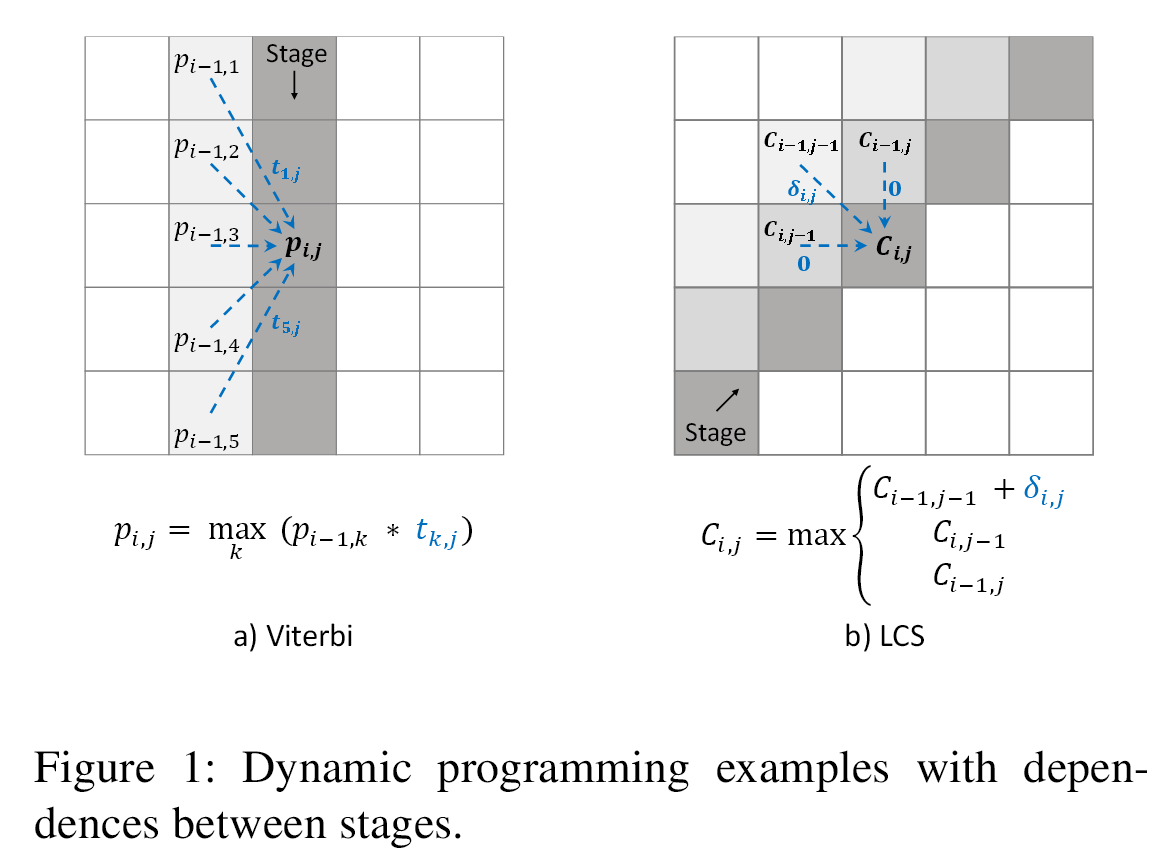
\includegraphics[scale=0.20]{figure/fig-wavefront-dp.png}
	\end{figure}
\end{frame}
\section{Parallel Design}

\subsection{Serial VGLCS Algorithm}
\begin{frame}
	\frametitle{Serial VGLCS Algorithm}
	\begin{figure}
		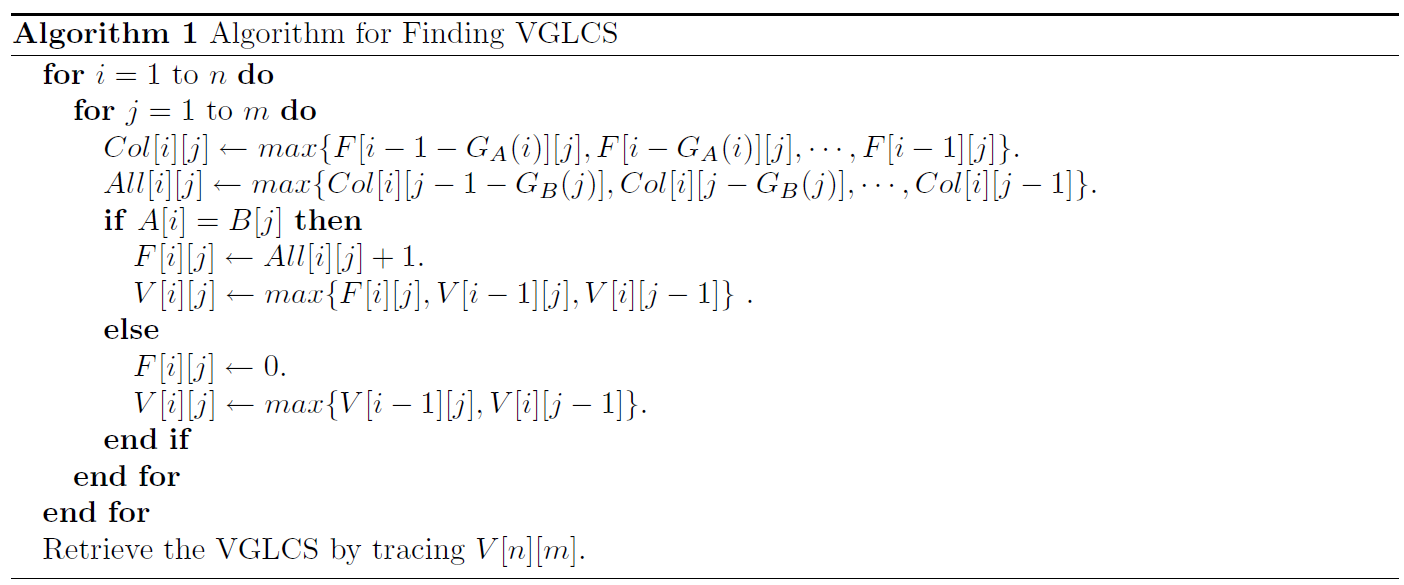
\includegraphics[scale=0.3]{figure/fig-VGLCS-algo.png}
	\end{figure}
\end{frame}

\subsection{Data Structure}
\begin{frame}
    \frametitle{Data Structure}
    \begin{itemize}
    \setlength\itemsep{1em}
    	\item Incremental Suffix Maximum Query
    		\begin{itemize}
    			\setlength\itemsep{1em}
    			\item Binary Indexed Tree (Fenwick Tree): $\mathcal{O}(\log n)$
    			\item Segment Tree: $\mathcal{O}(\log n)$
    			\item Van Emde Boas Tree: $\mathcal{O}(\log \log n)$
    			\item Disjoint Set: $\Omega(\alpha(n))$
    			\item Sparse Table: $\mathcal{O}(n \log n)$ - $\mathcal{O}(1)$
    		\end{itemize}
    	\item Which one is cache-friendly/ exploit parallelism easily?
    \end{itemize}
\end{frame}

\subsection{Hybrid Stages}
\begin{frame}
	\frametitle{Data Dependency}
	\begin{itemize}
		\setlength\itemsep{1em}
		\item We want to remove \texttt{All[i][j]} because its data dependency 
			is hard to parallel.
		\item The $O(n \log n)$ - $O(1)$ sparse table is a good alternative plan. 
		\item However, parallel algorithm will be $O(n^2 \max(\log n, \alpha(n)) / p + n \max(\log n, \alpha(n)))$ 
			with $p$ processors.
	\end{itemize}
\end{frame}

\begin{frame}
	\frametitle{Parallel VGLCS Algorithm}
\end{frame}

\begin{frame}
	\frametitle{Workload Imbalance}
	\begin{itemize}
		\setlength\itemsep{1em}
		\item Disjoint set has a lot of indirect jumps, and it leads cache miss penatly.
		\item Due to the compensatory hardware threading and L2 cache layout, affinity 
			is important on the MIC. We can control of thread affinity via \tt{KMP\_AFFINITY}
	\end{itemize}
\end{frame}

\begin{frame}
	\frametitle{Improve Workload (TODO)}
	\begin{itemize}
		\setlength\itemsep{1em}
		\item Reduce cache miss
			\begin{itemize}
				\setlength\itemsep{1em}
			 	\item Relayout data of disjoint set: structure of array, 
			 		array of structure, hybrid combinations, or ...
			 	\item Software caches
			 	\item Data compression
			\end{itemize}
		\item Reduce indirect jumps
			\begin{itemize}
				\setlength\itemsep{1em}
				\item The policy of path compression / union by rank
			\end{itemize}
	\end{itemize}
\end{frame}

\begin{frame}
	\frametitle{Exploit Parallelism (TODO)}
	\begin{itemize}
		\item Using rank convergence in dynamic programming algorithm
			\footnote{Paper: Efficient Parallelization Using Rank Convergence in 
				Dynamic Programming Algorithm}
	\end{itemize}
\end{frame}

\subsection{Serial part-VG LCS Algorithm (TODO)}
\begin{frame}
	\frametitle{Serial part-VG LCS Algorithm}
\end{frame}

\subsection{Parallel part-VG LCS Algorithm (TODO)}
\begin{frame}
	\frametitle{Parallel part-VG LCS Algorithm}
\end{frame}

\subsection{Optimization (TODO)}
\begin{frame}
	\frametitle{Optimization (TODO)}
	\begin{itemize}
		\item Coalesced memory access or memory coalescing
			\begin{itemize}
				\item Doubling algorithm creates smaller table
					and uses more computation in query.
			\end{itemize}
	\end{itemize}
\end{frame}
\section{Experiment}

\subsection{Environment Settings}
\begin{frame}
    \frametitle{Environment}
\end{frame}

\subsection{Result}
\begin{frame}
    \frametitle{Speedup}
    \begin{table}
    	\caption{$n = 5000, \; \forall G[i] < 10$}
		\begin{tabular}{| l | l | l | l |}
			\hline
			Algorithm 		& n = 5000 & n = 2000 & n = 1000\\ \hline
			serial 			& 1.172 & 0.190 & 0.044\\ \hline
			parallel 	& 0.218 & 0.077 & 0.033\\ \hline
		\end{tabular}
	\end{table}
\end{frame}

\begin{frame}
    \frametitle{Scalability}
    \begin{table}
    	\caption{$n = 5000$}
		\begin{tabular}{| l | l | l | l | l |}
			\hline
			Algorithm 	& p = 1 & p = 2 & p = 4 & p = 8\\ \hline
			parallel 	& 0.928  & 0.508 & 0.303 & 0.240 \\ \hline
		\end{tabular}
	\end{table}
\end{frame}
\section{Conclusion}

\subsection{Conclusion}
\begin{frame}
    \frametitle{Conclusion}
    \begin{itemize}
    	\setlength\itemsep{1em}
    	\item
    		VGLCS problem
    		\begin{itemize}
    			\setlength\itemsep{1em}
    			\item 
                    East-to-implements linear sparse table as
                    rightmost-pops encoding sparse table runs in $O(n^2
                    s/p+n\;\max(\log n, s))$.
				\item
					It can be solved in theorem $O(n^2/p+n\log n)$
		    		efficiently.
    		\end{itemize}
    	\item
    		Incremental ranged maximum query
    		\begin{itemize}
    			\setlength\itemsep{1em}
    			\item
    				It is more powerful than the incremental suffix
					maximum query.
				\item
					It can be solved in amortized $O(1)$ by our sparse
					table.
    		\end{itemize}
    \end{itemize}
\end{frame}
%\appendix
\section{Progress}

\subsection{Prerequisites}
\begin{frame}
    \frametitle{All Pair Least Common Ancestors}
    \begin{itemize}
    	\setlength\itemsep{1em}
    	\item Generating all binary search tree(BST) from $1$ to $n$.
    	\item Store $\textit{LCA}(p, q)$ with node $p$ and $q$ for each BST $T$.
		\item The size of table is $\theta(n^2 \frac{1}{n+1} \binom{2n}{n})$.
		\item We need real-time encoding-decoding. Therefore, 
			each step consumes $\mathcal{O}(1)$ time, 
			and total time is $\mathcal{\theta}(n)$.
    \end{itemize}
\end{frame}

\subsection{Parallel Generating All BST}
\begin{frame}
	\frametitle{Identity for BST}
		\tikzset{
  treeInode/.style = {align=center, inner sep=1pt, text centered,
    font=\sffamily},
  arn_n/.style = {treeInode, rectangle, rounded corners=1mm, black, draw=black, fill=black, text=white, font=\sffamily\bfseries, minimum width=1em, minimum height=1em}
    % arbre rouge noir, noeud noir
}
\usetikzlibrary{patterns}

\begin{tikzpicture}[-,>=stealth',level/.style={sibling distance = 0.5cm/#1,
  level distance = 0.6cm}]
\node[arn_n]{0}
; 
\node[below=0.2cm, align=flush center,text width=1cm]{$0$};
\end{tikzpicture}
		\begin{tikzpicture}[-,>=stealth',level/.style={sibling distance = 0.6cm,
  level distance = 0.4cm}]
\node[arn_n]{\tiny $1$}
  child{
    node[arn_n]{\tiny $0$}
  }
  child[missing]{
  }
; 
\node[below=1cm, align=flush center,text width=1cm]{\small $0$};
\end{tikzpicture}
\begin{tikzpicture}[-,>=stealth',level/.style={sibling distance = 0.6cm,
  level distance = 0.4cm}]
\node[arn_n]{\tiny $0$}
	child[missing]{
	}
	child{
		node[arn_n]{\tiny $1$}
	}
; 
\node[below=1cm, align=flush center,text width=1cm]{\small $1$};
\end{tikzpicture}
		\begin{tikzpicture}[-,>=stealth',level/.style={sibling distance = 0.5cm/#1,
  level distance = 0.6cm}] 
\node[arn_n]{2}
  child{
    node[arn_n]{1}
    child{
      node[arn_n]{0}
    }
    child[missing]{
    }
  }
  child[missing]{
  }
; 
\node[below=1.5cm, align=flush center,text width=0.5cm]{$0$};
\end{tikzpicture}
\begin{tikzpicture}[-,>=stealth',level/.style={sibling distance = 0.5cm/#1,
  level distance = 0.6cm}] 
\node[arn_n]{2}
  child{
    node[arn_n]{0}
    child[missing]{
    }
    child{
      node[arn_n]{1}
    }
  }
  child[missing]{
  }
; 
\node[below=1.5cm, align=flush center,text width=0.5cm]{$1$};
\end{tikzpicture}
\begin{tikzpicture}[-,>=stealth',level/.style={sibling distance = 0.5cm/#1,
  level distance = 0.6cm}] 
\node[arn_n]{1}
  child{
    node[arn_n]{0}
  }
  child{
    node[arn_n]{2}
  }
; 
\node[below=1.5cm, align=flush center,text width=0.5cm]{$2$};
\end{tikzpicture}
\begin{tikzpicture}[-,>=stealth',level/.style={sibling distance = 0.5cm/#1,
  level distance = 0.6cm}] 
\node[arn_n]{0}
  child[missing]{
  }
  child{
    node[arn_n]{2}
    child{
      node[arn_n]{1}
    }
    child[missing]{
    }
  }
; 
\node[below=1.5cm, align=flush center,text width=1cm]{$3$};
\end{tikzpicture}
\begin{tikzpicture}[-,>=stealth',level/.style={sibling distance = 0.5cm/#1,
  level distance = 0.6cm}] 
\node[arn_n]{0}
  child[missing]{
  }
  child{
    node[arn_n]{1}
    child[missing]{
    }
    child{
      node[arn_n]{2}
    }
  }
; 
\node[below=1.5cm, align=flush center,text width=0.5cm]{$4$};
\end{tikzpicture}
\end{frame}

\end{document}
